\documentclass[11pt]{article}
%Gummi|065|=)

\usepackage[utf8]{inputenc}
\usepackage[english]{babel}
\usepackage{graphicx}

\graphicspath{ {images/} }

\title{\textbf{Project Description for the summer course TIG-055}}
\author{Andreas Löfman\\
				Felix Bärring\\}
\date{2014-06-23}
\begin{document}

\maketitle

\section*{Abstract}

We want to create an application for the android system so that the user can connect a phone or tablet to a PC(Linux/Mac/Windows) and be able to send mouse and keyboard events. Essentially the android device will act as a controller for the PC. The android application will feature a GUI that provides easy means to control the the desktop computer, consisting of a qwerty keyboard and a rectangular area for a track-pad. We might also attempt to use the gyro functionality to control the mouse, depending on our overall progress.

\section*{Technical Details} 

To achieve our goals we will need to implement the following features.

\begin{itemize}
\item {
An android application that have an easy to use GUI consisting of four views. One for keyboard and for track  pad as well as a view for settings and connection to a java server. There will also be a special view which only consist of the necessary keys for gaming, i.e it will remove the most of the typing keys to make it a more streamlined design like a game-pad.




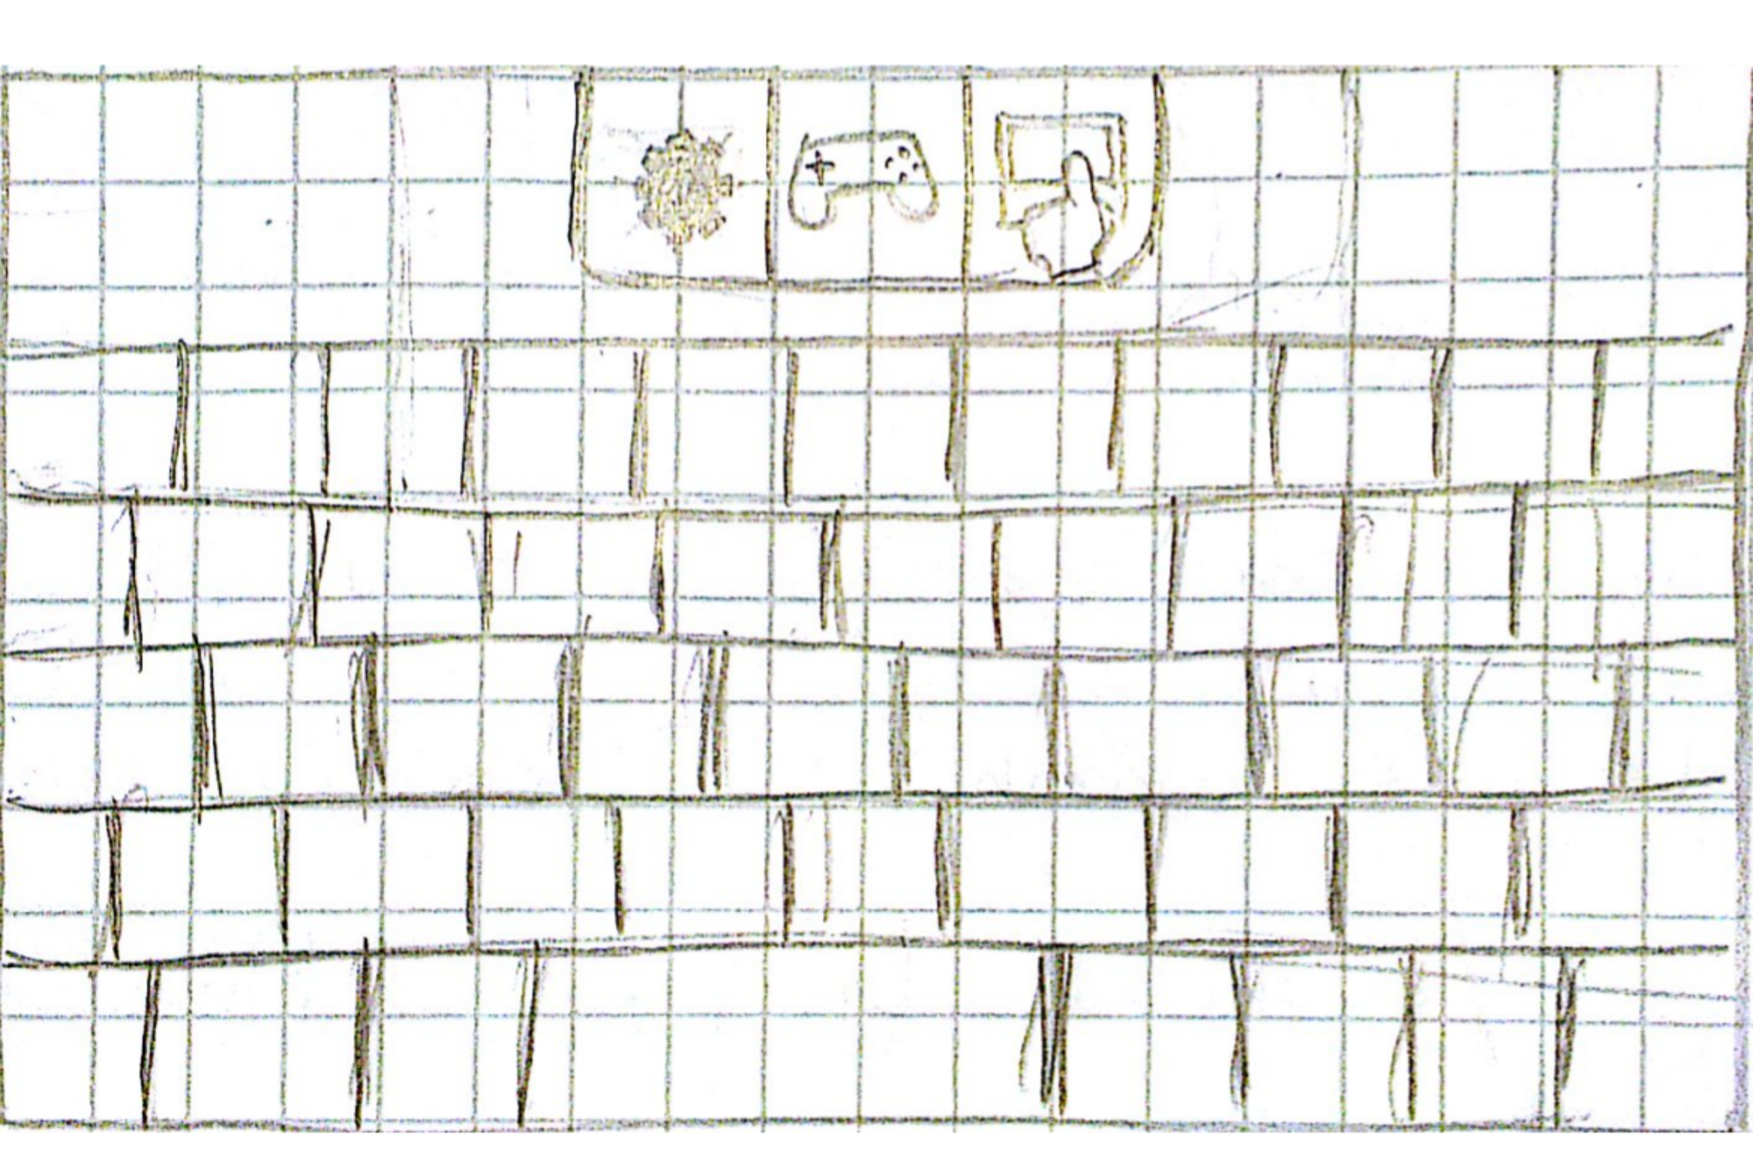
\includegraphics[scale=0.2]{keyboardView}

Keyboard View

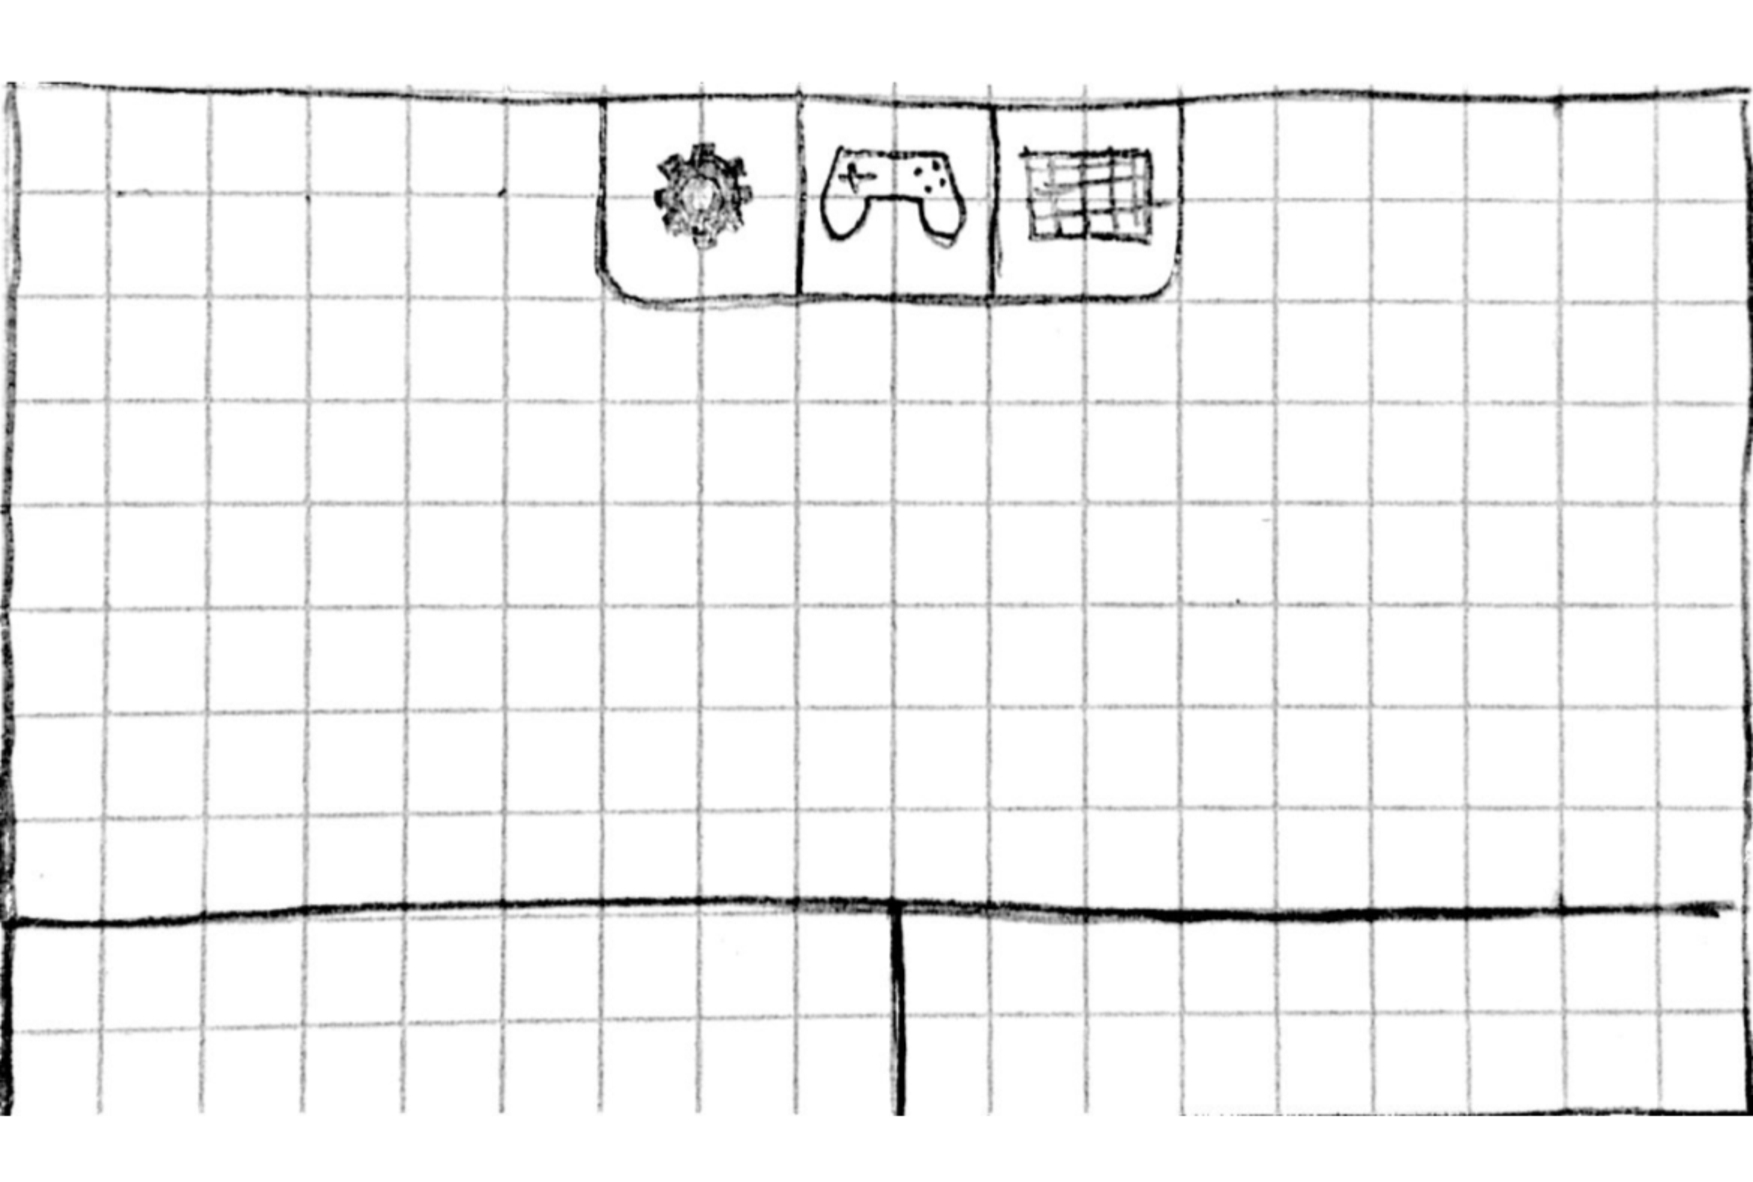
\includegraphics[scale=0.2]{touchpadView}

Touchpad View

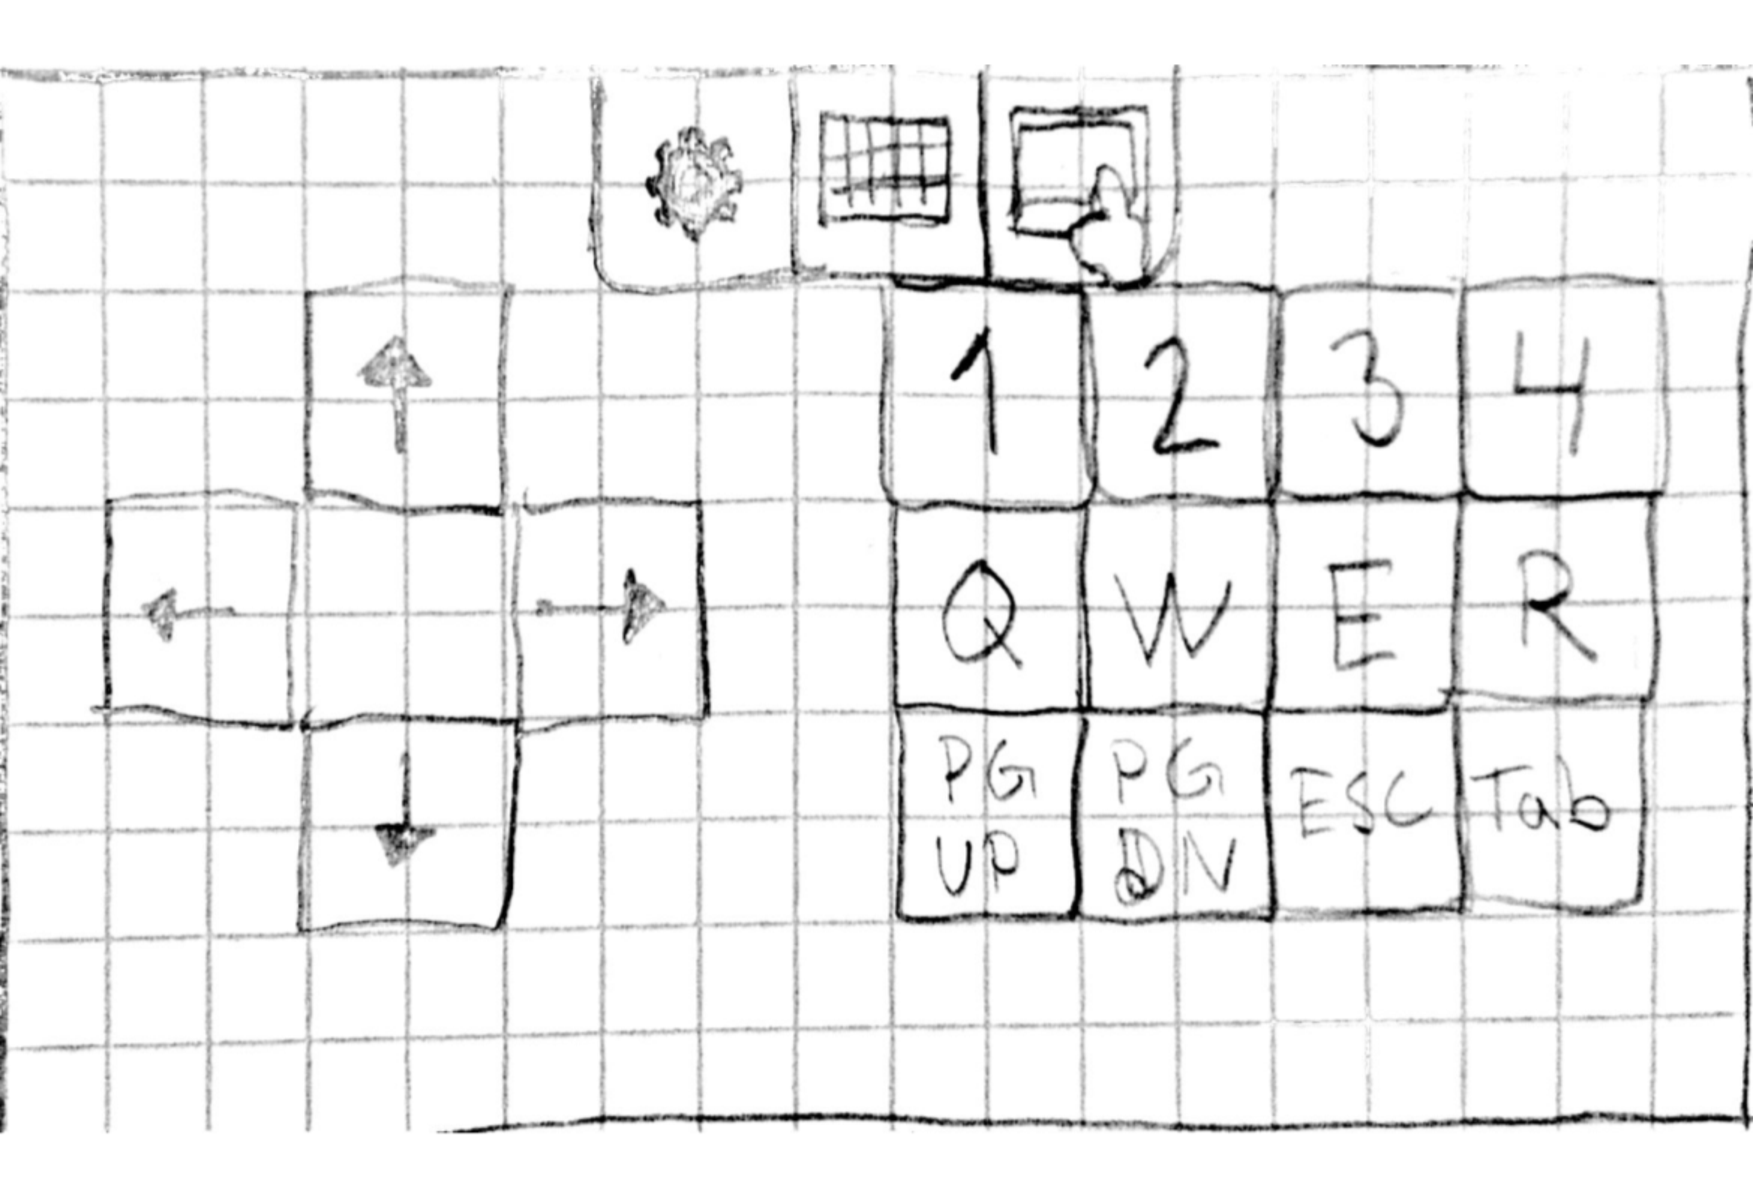
\includegraphics[scale=0.2]{gamingView}

Gamming View

%%Pictures here

}

\item {
A java server that is responsible for the communication between the PC and the android device. We will be using server sockets that will be listening for the connection from the android device, only one connection will be allowed at one time. The server will be receiving messages containing keyboard/mouse events and handle them appropriately. Our initial approach to generate system key/mouse events will be to use java.awt.Robot class which should be a good starting point. If time permits we will try to research and implement platform specific solutions using Java Native Interface.
}


\item {
On the PC we will use a simple SWING GUI that will be used to set a server port and start the server. It will also have an output window that presents the input that the server receives so that the user can easily see what is going on.
}

\end{itemize}

\end{document}
